\documentclass[10pt,letterpaper,twocolumn]{article}

\usepackage[top=2.1cm,left=2.0cm,right=2.0cm,footskip=2.0cm]{geometry}
\usepackage[utf8]{inputenc}     % for Unicode
\usepackage{cite}               % citation
\usepackage[dvipdfmx]{hyperref} % links
\usepackage{caption}            % caption
\usepackage{microtype}          % improves typesetting in LaTeX
\usepackage{algpseudocode}
\usepackage{algorithm}
\usepackage{graphicx}
\usepackage{color} % ex.) \textcolor{color}{text}
\usepackage{lipsum}

\newcommand\blfootnote[1]{%
    \begingroup
    \renewcommand\thefootnote{}\footnote{#1}%
    \addtocounter{footnote}{-1}%
    \endgroup
}
\renewcommand{\algorithmicrequire}{\textbf{Input:}}
\renewcommand{\algorithmicensure}{\textbf{Output:}}

\begin{document}

\twocolumn[
    \begin{flushleft}
        {\Large
        \textbf\newline{An Extention of R-Tree for Periodic Boundary Conditions}
        }
        \newline
        \\
        Toru Niina \textsuperscript{1}
        \\
        \bigskip
        \bf{1.} Department of Biophysics, Graduate School of Science,
                Kyoto University, Kyoto 606-8502, Japan
        \\
        \bigskip
        * niina@theory.biophys.kyoto-u.ac.jp
    \end{flushleft}

    \section*{Abstract}
    Searching spatial data is an important operation for scientific simulations
    which are performed mostly on periodic boundary conditions.
    An R-Tree is a widely used tree data structure to manage spatial objects and
    it is capable of answering to spatial searching queries in an efficient way.
    In this paper, I propose a new method to construct R-Tree along the periodic
    boundary conditions by introducing a set of operations for rectangles.
    Unlike existing methods, this method works without any kind of additional
    copies of objects or queries.
    Moreover, because this method reduces the size of bounding boxes for each
    nodes of R-Tree in the natural way along the periodic boundary conditions,
    it is expected to increase the efficiency of processing spatial queries.
    The method can essentially be applied not only to Guttman's original R-Tree
    but also to the other kind of algorithm if it handles recutangles on the
    periodic boudary conditions. The implementation is available on GitHub.
    \bigskip
]


\section*{Introduction}

Computational simulations are the essential tools for scientific research, such
as investigating behaviors of complex biochemical models. To perform such a large
scale simulation, both huge amount of computational resources and efficient
simulation softwares are required.
\blfootnote{
This paper is distributed under a Creative Commons BY-NC-ND.
To see the full text of the license, see
https://creativecommons.org/licenses/by-nc-nd/4.0/legalcode.
}

In most cases, searching for objects that satisfy some geometrical conditions
is one of the most costly operation in the simulation. Generally, an efficient
method for spatial search drastically accelerates not only the whole simulation
processes, but also the data analysis of simulation results. Therefore, a method
that accelerates spatial searching also accelerates whole process of scientific
simulation research.

An R-Tree is a widely used data structure representing bounding volume
hierarchies (BVH) by using axis-aligned bounding box (AABB) for all its entries
\cite{Guttman1984}. It is capable of containing both sizeless and finite sized
objects such as points, segments, spheres and etc. As its efficiency, many
variants have been proposed and are applied for many problems in a broad range
of fields.

In order to use it with periodic boundary conditions (PBCs), currently,
two methods are proposed (figure\ref{fig1})\cite{CoSTR-R-tree2016}.
The method visually described in figure \ref{fig1}A copies all the objects in
the simulation system along each periodic boundaries.
Although it can search objects associated with the adjacent periodic images in
the same way as normal R-Tree, it consumes memory $3^D$ fold a lot (here $D$
reprecents a number of dimension).
Figure \ref{fig1}B showes another method that contains only one image,
copying query AABB in the same manner as copying whole system if the query goes
outside of the boundary.
Although it works completely fine with sizeless particles, it has a problem to
contain finite-sized objects. It might overlook objects if query is not copied
when the query is inside of the boundary and objects extends beyond the unit
cell (figure\ref{fig1}C).

Here I propose the novel method to apply PBCs to R-Tree. The main idea is
applying the PBCs to each operations for AABBs that are performed in each steps
to maintain an R-Tree. Allowing the AABBs of each nodes to extend in a periodic
manner, the R-Tree become capable of containing objects in the most natural way
on PBCs to overcome the limitation of containing finite sized object
(figure\ref{fig1}CD). With this method, it is not needed to copy objects
or queries at all. Moreover, using the information about the boundary condition,
it is expected that the size of each AABBs associated with each nodes decreases
relative to the other methods, suggesting that the spatial search become more
efficient.

\begin{figure}[hbt]
    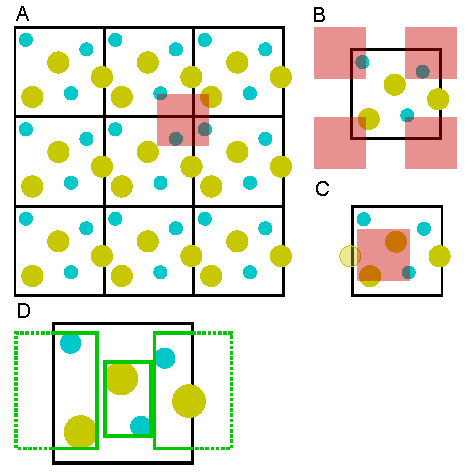
\includegraphics[width=8.4cm, bb=6 3 220 224]{fig1.eps}
    \caption{Methods to handle R-Tree on periodic boundary conditions.
    (\textbf{A})
    By copying the unit cell for each dimension along periodicity, normal R-Tree
    can manage objects that are associated with periodic images.
    (\textbf{B})
    By adding extensional query translated for each periodic images, R-Tree can
    detect objects that are beyond boundary.
    (\textbf{C})
    With the method described in \textbf{B}, finite sized objects could be
    overlooked when queries that is inside of the boundary are not copied.
    (\textbf{D})
    This is the method proposed in this paper. Forming rectangles according to
    the periodicity, R-Tree can organize objects on periodic boundary
    conditions.}
    \label{fig1}
\end{figure}

\section*{Methods}

The operations that are provided in this paper is for handling and modifying
AABBs on PBCs.
I do not modify the algorithm to grow and maintain an R-Tree at all.
Hence, in this setion, I do not show algorithm to construct R-Tree itself.
The main algorithm used to make an R-Tree for performance measuring is
completely same as original Guttman's quadratic algorithm.
It means that the operations can potentially be applied for some of the R-Tree
variants and the other spatial indexing methods that uses AABBs.

Because the rectangles that are used in R-Tree are axis-aligned, it is
enough to show the operation for one dimension to provide the whole algorithm.
Applying those procedure to each dimensions successively, these operations can
easily be extended for higher dimension cases.

\paragraph{Representation of the PBCs.}
As an unit cell of the PBCs, I consider only cuboids so that it become
drastically easier to handle rectangles on the condition.
I restrict coordinates of all the objects to inside of the unit cell.
There are well-known alrogithm to restrict coordinates and vectors to the unit
cell. In this paper, I call them as \textbf{RestrictPosition} and
\textbf{RestrictVector}, respectively.

\paragraph{Representation of an rectangles.}
There are some options to represent an rectangle such as a pair of coordinates
describing upper and lower limit in each dimensions, a pair of coordinate and
vector describing its characteristic position and width of rectangle in each
dimension. Because the method proposed in this paper quite often uses centroids
of rectangles, here I represent a rectangle as a pair of centroid position and
width vector (figure \ref{fig2}).

\begin{equation}
    rectangle = \{centroid, width\}
\end{equation}

Of course, all the representations have identical information, one can easily
convert a certain representation to another.

\paragraph{Expanding AABBs on PBCs.}
Expanding an AABB to make it a minimal bounding box of its contents is one of
the most important operations done to form R-Tree.
Because the total area that is covered by AABBs in the nodes of R-Tree affects
the efficiency of spatial searching, it is needed to find the way to make the
expanded area as small as possible.

The algorithm to find the minimum expansion of AABB to contain another AABB on
PBCs is shown in algorithm ~\ref{expand_aabb_aabb}.
The size of bounding box that contains two rectangles is determined by the
distance between their centroids (figure \ref{fig-expand-box}).
Therefore, by restricting the vector between centroids, the minimum expansion
can be found.

\begin{algorithm}
    \caption{expand AABB so that it contains another AABB}
    \label{expand_aabb_aabb}
    \begin{algorithmic}
        \State $R1 \gets$ original rectangle
        \State $R2 \gets$ rectangle to contain
        \State $B  \gets$ boundary
        \Function{ExpandAABB}{$R1, R2, B$}
            \State $dc \gets R2.centroid - R1.centroid$
            \State $dc \gets$ \Call{RestrictVector}{dc, B}

            \State $l1 \gets R1.centroid - R1.width / 2$
            \State $u1 \gets R1.centroid + R1.width / 2$
            \State $l2 \gets (R1.centroid + dc) - R2.width / 2$
            \State $u2 \gets (R1.centroid + dc) + R2.width / 2$

            \State $L \gets min(l1, l2)$
            \State $U \gets max(u1, u2)$
            \State $C \gets (L + U) / 2$
            \State $W \gets U - L$

            \State $C \gets$ \Call{RestrictPosition}{C, B}
            \State \Return $\{C, W\}$
        \EndFunction
     \end{algorithmic}
\end{algorithm}

For the case of containing points, it become simpler as described in the
algorithm ~\ref{expand_aabb_point}.

\begin{algorithm}
    \caption{expand AABB so that it contains a point}
    \label{expand_aabb_point}
    \begin{algorithmic}
        \State $R \gets$ original rectangle
        \State $P \gets$ point
        \State $B \gets$ boundary
        \Function{ExpandAABB}{$R, P, B$}
            \State $dc \gets P - R.centroid$
            \State $dc \gets$ \Call{RestrictVector}{dc, B}

            \State $l \gets R.centroid - R.width / 2$
            \State $u \gets R.centroid + R.width / 2$

            \State $L \gets min(l, P)$
            \State $U \gets max(u, P)$
            \State $C \gets (L + U) / 2$
            \State $W \gets U - L$

            \State $C \gets$ \Call{RestrictPosition}{C, B}
            \State \Return $\{C, W\}$
        \EndFunction
     \end{algorithmic}
\end{algorithm}

\paragraph{Detecting an object includes or intersects the other object}

To find an object in an R-Tree, it is needed to check an object is inside of
an rectangle. Whether an object includes or intersects the other object can be
determined by using the minimum distance between centroids of the objects.
Figure ~\ref{fig-geometrical-relationship} graphically shows the idea of each
algorithms in 1 dimension.

\begin{algorithm}
    \caption{Check whether an AABB is inside of an AABB}
    \begin{algorithmic}
        \State $R1 \gets$ rectangle
        \State $R2 \gets$ rectangle that might be inside of R1
        \State $B  \gets$ boundary
        \Function{IsAABBInsideOfAABB}{$R1, R2, B$}
            \State $dc \gets R1.centroid - R2.centroid$
            \State $dc \gets$ \Call{RestrictVector}{dc, B}

            \State \Return $\mathrm{abs}(dc) \leq (R1.width - R2.width) / 2$
        \EndFunction
     \end{algorithmic}
\end{algorithm}

\begin{algorithm}
    \caption{Check whether a point is inside of an AABB}
    \begin{algorithmic}
        \State $R \gets$ rectangle
        \State $P \gets$ point
        \State $B \gets$ boundary
        \Function{IsPointInsideOfAABB}{$R, P, B$}
            \State $dc \gets R.centroid - P$
            \State $dc \gets$ \Call{RestrictVector}{dc, B}
            \State \Return $\mathrm{abs}(dc) \leq (R.width) / 2$
        \EndFunction
     \end{algorithmic}
\end{algorithm}

\begin{algorithm}
    \caption{Check whether an AABB intersects to another AABB}
    \begin{algorithmic}
        \State $R1 \gets$ rectangle
        \State $R2 \gets$ rectangle that might intersect to R1
        \State $B  \gets$ boundary
        \Function{IsAABBIntersectsAABB}{$R1, R2, B$}
            \State $dc \gets R.centroid - R.centroid$
            \State $dc \gets$ \Call{RestrictVector}{dc, B}
            \State \Return $\mathrm{abs}(dc) \leq (R1.width + R2.width) / 2$
        \EndFunction
     \end{algorithmic}
\end{algorithm}

\section*{Results}

The codes that are used in this paper can be found in GitHub
\cite{periortree-implementation}.

\paragraph*{performance measurements}
Lorem ipsum dolor sit amet, consectetur adipiscing elit. Aliquam bibendum
finibus diam, gravida sagittis lorem gravida vitae. Interdum et malesuada fames
ac ante ipsum primis in faucibus. Nulla in diam tristique ante posuere
tristique. Donec interdum purus sit amet nisl accumsan consectetur. Fusce
aliquet libero mi, quis ornare dolor congue ullamcorper. Nulla nulla urna,
molestie in urna sed, lacinia volutpat eros. Ut mi libero, elementum scelerisque
ipsum vel, hendrerit fermentum turpis. Aliquam sit amet leo sodales, egestas
augue id, fermentum nulla. Aenean vel cursus ante, et pellentesque eros. Nulla
ac neque nec justo posuere commodo sit amet sit amet justo. Aliquam tincidunt
tempor ex nec tincidunt. In ullamcorper vehicula lobortis.

\section*{Conclusion}

In this paper, the novel method for applying PBCs to Guttman's R-Tree is
introduced. Proposed method is capable of containing not only sizeless points but also
objects with finite size. The method can remove the necessity of storing
extensional objects or replicating queries. Moreover, it reduces the size of
each node in the natural way on PBCs.

On the other hand, the method introduces tiny but additional costs into each
procedures for maintaining R-Tree and checking geometrical conditions because it
considers the PBCs for all of the procedure. It might decrease the efficiency of
the R-Tree in some case.

As described before, since the method is only for modifying and handling
rectangles on PBCs, it can essentially be applied for the other R-Tree variants
or the other kind of spatial indexing methods.

Because the adaptation of spatial indexing to a system on PBCs has a chance to
accelerate many kind of sientific simulations, it is expected that this novel
method will have an important role for the simulations that will be performed in
the next decade.

\bibliographystyle{plain}
\bibliography{library}{}

\end{document}
